\documentclass[../mathNotesPreamble]{subfiles}

\providecommand{\subfiles}{.}
\begin{document}
%  \relscale{1.4} %TODO
  \section{4.2: Measuring Strength of Association with Correlation}
    \begin{defn*}
      The \textbf{correlation coefficient} is a number that measures the strength of the linear association between two numerical variables. The correlation coefficient is between $-1$ and $1$:
      \begin{center}
        \begin{tabular}{@{}rl@{}}\toprule
          $1 \rightarrow$ & Strong association and positive trend\\
          $0 \rightarrow$ & Weak or no association\\
          $-1 \rightarrow$ & Strong association and negative trend\\\bottomrule
        \end{tabular}
      \end{center}
      \emph{The correlation coefficient only makes sense if the trend is linear and both variables are numerical!!}
    \end{defn*}
    \vspace*{\stretch{1}}

    \begin{center}
      Note: \emph{Correlation does not mean causation!}\\[\baselineskip]
      
      Take a few minutes to look at the graphs at this link: \href{https://www.tylervigen.com/spurious-correlations}{\textcolor{blue}{\underline{Spurious correlations}}}\\[\baselineskip]
      
      \href{https://xkcd.com/552}{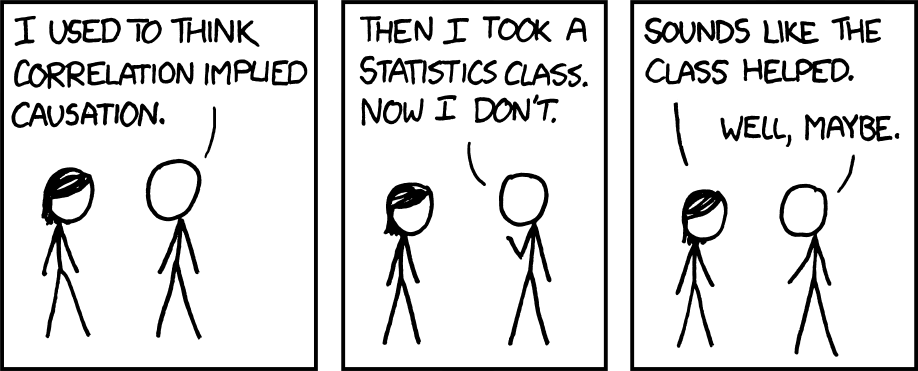
\includegraphics[width=0.85\linewidth]{images/correlation_2x_xkcd_552}}
    \end{center}
    \pagebreak
    
    \vspace*{\stretch{1}}
    \begin{center}
      \begin{tikzpicture}[nodes=black]
        \begin{groupplot}[
          group style={group size=2 by 2, horizontal sep=2cm},
          axis lines=center,
          axis line style={black,->},
          enlargelimits={value=0.025, auto},
          width=0.45\linewidth, height=0.3\linewidth,
          ticklabel style={font=\footnotesize,inner sep=0.5pt,fill=white,opacity=1.0, text opacity=1},
          xlabel style={at={(ticklabel* cs:0.5)},anchor=north, yshift=-10pt},
          ylabel style={at={(ticklabel* cs:0.5)},anchor=south, xshift=-27.5pt, rotate=90},
          ]
            \nextgroupplot[xlabel=Height (inches), ylabel=Height (cm)]
              \addplot[only marks, blue] table [x=Height, y=HTCm, col sep=comma] {\subfiles/scat_plot_data_4p2.csv} node at(62,190) {$r=1.00$};
            \nextgroupplot[xlabel=Height (inches) , ylabel=Weight (lbs)]
              \addplot[only marks, blue] table [x=Height, y=Weight, col sep=comma] {\subfiles/scat_plot_data_4p2.csv} node at(61,230) {$r=0.72$};
        \end{groupplot}
      \end{tikzpicture}
      \vspace*{\baselineskip}
      
      \begin{tikzpicture}[nodes=black]
        \begin{axis}[
          axis lines=center,
          axis line style={black,->},
          xmin=15, xmax=65,
          ymin=-4.25, ymax=4.25,
          enlargelimits={value=0.025, auto},
          width=0.55\linewidth, height=0.3\linewidth,
          ticklabel style={font=\footnotesize,inner sep=0.5pt,fill=white,opacity=1.0, text opacity=1},
          xlabel=Age (years), xlabel style={at={(ticklabel* cs:0.5)},anchor=north, yshift=-30pt},
          ylabel=Time (hours), ylabel style={at={(ticklabel* cs:0.5)},anchor=south, xshift=-20pt, rotate=90},
          ]
            \addplot[only marks, blue] table [x=x_sim, y=y_sim, col sep=comma] {\subfiles/scat_plot_data_4p2.csv} node at (47.5,3.2) {$r=0$};
        \end{axis}
      \end{tikzpicture}
      \vspace*{\baselineskip}
      
      \begin{tikzpicture}[nodes=black]
        \begin{groupplot}[
          scaled ticks=false,
          group style={group size=2 by 2, horizontal sep=2cm},
          axis lines=center,
          axis line style={black,->},
          enlargelimits={value=0.025, auto},
          width=0.45\linewidth, height=0.3\linewidth,
          ticklabel style={font=\footnotesize,inner sep=0.5pt,fill=white,opacity=1.0, text opacity=1},
          xlabel style={at={(ticklabel* cs:0.5)},anchor=north, yshift=-10pt},
          ylabel style={at={(ticklabel* cs:0.5)},anchor=south, xshift=-27.5pt, rotate=90},
          ]
            \nextgroupplot[xlabel=Age, ylabel=Price]
              \addplot[only marks, blue] table [x=age, y=price, col sep=comma] {\subfiles/scat_plot_data_4p2.csv} node at (33,25000) {$r=-0.50$};
            \nextgroupplot[xlabel=Age, ylabel=Year]
              \addplot[only marks, blue] table [x=age, y=year, col sep=comma] {\subfiles/scat_plot_data_4p2.csv} node at (33,2005) {$r=-1.00$};
        \end{groupplot}
      \end{tikzpicture}
    \end{center}
  \vspace*{\stretch{1}}
  \pagebreak
  
  \begin{defn*}
    The formula for the correlation coefficient between two variables $x$ and $y$ is
      \[r=\dfrac{\sum z_xz_y}{n-1}\]
    where $z_x$ and $z_y$ are the $z$ scores for each entry in the $x$ and $y$ lists.
      \[z_x=\dfrac{x-\overline{x}}{s_x} \qquad z_y=\dfrac{y-\overline{y}}{s_y}\]
  \end{defn*}
  \begin{ex*}
    Below are the heights and weights of six women:
    \begin{center}
      \begin{tabular}{@{}l*{6}{c}@{}}\toprule
        Heights& 61& 62& 63& 64& 66& 68\\
        Weights& 104& 110& 141& 125& 170& 160\\\bottomrule
      \end{tabular}
    \end{center}
    Compute the correlation coefficient by hand. Then, graph the scatterplot and compute the correlation coefficient using StatCrunch.
  \end{ex*}
  \vspace*{\stretch{1}}
  \begin{flushright}
    \begin{tikzpicture}[nodes=black]
      \begin{axis}[
        axis lines=center,
        axis line style={black,->},
        enlargelimits={value=0.05, auto},
        ticklabel style={font=\footnotesize,inner sep=0.5pt,fill=white,opacity=1.0, text opacity=1},
        xlabel=Height (in), xlabel style={at={(ticklabel* cs:0.5)},anchor=north, yshift=-10pt},
        ylabel=Weight (lbs), ylabel style={at={(ticklabel* cs:0.5)},anchor=south, xshift=-20pt, rotate=90},
        ]
          \addplot[only marks, blue] table [x=women_height, y=women_weight, col sep=comma] {\subfiles/scat_plot_data_4p2.csv};
      \end{axis}
    \end{tikzpicture}
  \end{flushright}
  \pagebreak
  
  \noindent\textbf{Understanding the Correlation Coefficient:}
  \begin{itemize}
    \item Changing the order of the variables does not change $r$
    \item Adding a constant or multiplying by a positive constant does not affect $r$
    \item The correlation coefficient is unitless
    \item None of this makes any sense if the relationship between the variables is not linear!
  \end{itemize}

  \pagebreak
\end{document}
